% ============================================================
\chapter{トラッキングエラーと情報レシオ}\label{ch:te}

機関投資家の運用の多くは、ベンチマーク（市場の指数など）に対して、どれだけ上回るかで評価される。そのとき、リスクは比率の絶対的な散らばりではなく、ベンチマークからのずれ（トラッキングエラー、TE）で測る。BL の結果は、時価総額の比率からの「能動的な傾き」なので、TE の言葉と相性がよい。この章では、TE と情報レシオ（IR）を BL と組み合わせる方法と、その落とし穴をまとめる。

\section{能動運用の言葉}

ベンチマークの比率を $w_b$、ポートフォリオの比率を $w$ とし、差 $w_a=w-w_b$ を能動的な比率と呼ぶ。

\begin{center}
\small
\begin{tabular}{p{2.8cm}p{4.2cm}p{6.0cm}}
\toprule
量 & 式 & 意味 \\
\midrule
超過リターン & $w_a\T r$ & ベンチマークをどれだけ上回ったか \\
期待超過リターン & $w_a\T\alpha$ & 期待で何 \% 上回るか（$\alpha$ はベンチマークに対する期待リターンのずれ） \\
トラッキングエラー & $\sqrt{w_a\T\Sigma w_a}$ & 超過リターンの標準偏差 \\
情報レシオ & $w_a\T\alpha/\sqrt{w_a\T\Sigma w_a}$ & TE 1 単位あたりの期待超過リターン \\
\bottomrule
\end{tabular}
\end{center}

事前（予想）の TE・IR と、事後（実績）の TE・IR は違う。事前の値はモデルの $\Sigma$ と $\alpha$ で計算し、事後の値は実際の超過リターンから計算する。両者がずれるのはふつうのことで、そのずれ方を確かめるのが大事である（\secref{sec:te-project}）。

\section{BL の結果は能動的な傾き}

制約のない最適化では、BL の比率は $w^*=\wmkt+P\T\Lambda$ だった（\secref{sec:hl-property}）。ベンチマークを時価総額の比率とすれば、能動的な比率は $P\T\Lambda$ で、ビューのポートフォリオの組み合わせになる。その TE は $\sqrt{\Lambda\T P\Sigma P\T\Lambda}$ である。Idzorek の例では、He--Litterman の $\Omega$ で TE は \V{idz.actrisk}\% だった（\chapref{ch:idzorek}）。

\section{TE を罰則にした最適化}

ビューから得た期待リターンのずれを $\alpha=\muBL-\Pi$ とし、能動的な比率を
\begin{equation}
\max_{w_a}\;w_a\T\alpha-\frac{\lambda_A}{2}w_a\T\Sigma w_a\qquad\text{s.t.}\quad \one\T w_a=0
\label{eq:active-opt}
\end{equation}
で決める。$\lambda_A$ は TE への回避度である。調査メモの目的関数 $w\T\muBL-\lambda_{TE}w_a\T\Sigma w_a$ も同じ形である。この問題は閉じた形で解ける（\appref{app:formulas}）。
\begin{equation}
w_a^*=\frac{1}{\lambda_A}h,\qquad h=\Sigma^{-1}\alpha-\frac{\one\T\Sigma^{-1}\alpha}{\one\T\Sigma^{-1}\one}\Sigma^{-1}\one
\end{equation}
$h$ の TE は、最大の情報レシオ
\begin{equation}
\IR^*=\sqrt{\alpha\T\Sigma^{-1}\alpha-\frac{(\one\T\Sigma^{-1}\alpha)^2}{\one\T\Sigma^{-1}\one}}
\label{eq:ir-star}
\end{equation}
に等しい。$\lambda_A$ を変えても、能動的な比率の向き $h$ は変わらず、大きさだけが変わる。TE の目標 $\TE^*$ を決めれば、$\lambda_A=\IR^*/\TE^*$、期待超過リターンは $\IR^*\cdot\TE^*$ である。

つまり、能動運用の最適化は 2 つの部分に分かれる。

\begin{enumerate}
\item \textbf{向き}：$\alpha$ と $\Sigma$ で決まる（ビューの中身）。
\item \textbf{大きさ}：TE の目標で決まる（どれだけずれてよいか）。
\end{enumerate}

BL の $\Omega$ や $\tau$ は、$\alpha$ の大きさを通じて $\IR^*$ を決める。ビューを信じすぎると $\alpha$ が大きくなり、事前の $\IR^*$ が大きく見える。

\section{TE だけで最適化すると、総リスクが増える}

Roll（1992）は、TE を最小にしながら期待超過リターンを最大にするポートフォリオ（TE の効率的フロンティア）が、平均分散の意味では効率的でなく、ベンチマークよりベータが大きく、総リスクも大きくなりやすいことを示した。期待リターンの高い資産は、多くの場合ベータも高いので、$\alpha$ に沿って傾けると、市場への露出も一緒に増えるためである。Jorion（2003）は、TE の制約に加えて総リスク（ポートフォリオのボラティリティ）の制約を置くことを勧めている。

Idzorek の例で確かめた。

\begin{table}[htbp]
\centering
\caption{Idzorek の例での能動運用の最適化。$\alpha=\muBL-\Pi$。「$\beta$ のずれ」は、TE 2\% の能動的な比率のベンチマークに対するベータ。右端は、ベータのずれを 0 にする制約を足した場合の最大の IR。}
\label{tab:te}
\tabin{te}
\end{table}

\tabref{tab:te} のとおり、この例では、能動的な比率のベータのずれは小さく（$\pm0.05$ 以内）、ベータを 0 に固定しても最大の IR はほとんど変わらない。ビューが債券と株式の両方にまたがり、ベータの高い資産だけに偏っていないためである。ビューが株式の一部に集中しているときは、ベータのずれを確かめる必要がある。

\subsection*{IR の値について}

He--Litterman の $\Omega$ で、最大の IR は \V{te.ir.hl} である。Idzorek の論文の表 8 の情報レシオ 0.0699 とは定義が違う。論文の値は、残差リターン（ベータで調整した超過リターン）を残差リスクで割ったもので、ポートフォリオの期待リターンには事後の値を、ベンチマークの期待リターンには均衡の値を使っている。この資料の値は、$\alpha=\muBL-\Pi$ を使い、ベンチマークに対する超過リターンを TE で割ったものである。どちらで測っても、この例のビューの事前の IR は 0.1 に届かない。

\section{TE をどうやって合わせるか}

TE を目標に合わせる方法は 2 つある。

\begin{description}[leftmargin=2em,style=nextline]
\item[$\tau$（や確信度）で合わせる] Lee（2000）の方法（Idzorek による紹介）や O'Toole（2017）の考え方。$\Omega$ を固定して $\tau$ を動かすと、BL の傾きの TE が変わる（\figref{fig:te} の左）。Idzorek の例では、$\tau=0.025$ で TE は \V{te.tau.base}\%、2\% にするには $\tau\approx\V{te.tau2}$ が必要である。
\item[最適化の制約で合わせる] $\Omega$ と $\tau$ はビューの当たり具合で決め、TE の大きさは最適化の制約（$\sqrt{w_a\T\Sigma w_a}\le\TE^*$）か罰則で決める。
\end{description}

\begin{figure}[htbp]
\centering
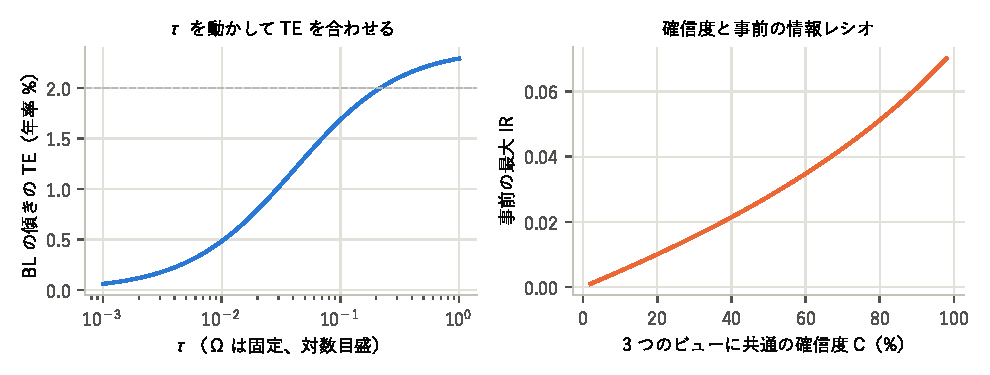
\includegraphics[width=0.95\linewidth]{fig_te.pdf}
\caption{Idzorek の例。左：$\Omega$ を固定して $\tau$ を動かしたときの、BL の傾きの TE。右：3 つのビューに共通の確信度 $C$（Idzorek の方法）と、事前の最大の IR。}
\label{fig:te}
\end{figure}

\figref{fig:te} の右のとおり、確信度を上げると事前の IR は上がる。確信度 50\% で \V{te.ir.c50}、90\% で \V{te.ir.c90} である。確信度を上げることは、TE を増やすだけでなく、「ずれ 1 単位あたりの見込み」も大きく見せる。$\tau$ で TE を合わせると、ずれの許容幅の都合で確信度を変えることになり、事前の IR が実力以上に大きく見えたり小さく見えたりする。この資料では、2 番目（$\Omega$ は当たり具合、TE は制約）を勧める。

\section{情報レシオの目安}

\begin{itemize}
\item Bevan と Winkelmann（1998）は、BL の比率の事前の IR が 2.0 を超えたら、ビューの重みを下げるよう勧めている（Idzorek による紹介）。
\item 実績の IR は、0.5 あれば優秀、1.0 なら例外的とされる。基本法則 $\IR\approx\IC\sqrt{\mathrm{BR}}$ で、IC 0.05 なら、独立な賭けが年に 100 回で IR 0.5 になる。
\item 事前の IR が 1 を大きく超えるなら、$\Omega$ が小さすぎる（ビューを信じすぎている）か、$\Omega$ を対角にして確信を積み上げている（\secref{sec:diag-trap}）可能性を疑う。
\end{itemize}

\section{本プロジェクトの TE}\label{sec:te-project}

\chapref{ch:project} で、本プロジェクトの LLM のビューを、較正した採用率で入れたうえで、事前の TE を年率 \V{bt.te.target}\% 以内にする制約を付けて最適化した。30 か月の実績の TE は \V{bt.fullte.te}\% で、目標を大きく上回った。制約を付けない場合の実績の TE は \V{bt.full.te}\% だったので、制約はずれを大きく減らしたが、目標どおりにはならなかった。

事前の TE が実績より小さく出るのは、次の理由による。

\begin{itemize}
\item 共分散は過去 252 日の縮小推定で、急な変動や個別の銘柄のニュースを捉えきれない。
\item 比率が毎月大きく入れ替わるので、月ごとに違う能動的な比率の TE を平均することになる。
\item 数百の銘柄に小さな比率を張ると、個別リスクの推定の誤差が積み上がる。
\end{itemize}

TE の制約を付けるときは、事前の目標を、実績が目標に収まるように控えめに置く（例えば実績の目標の半分程度）か、実績を見ながら調整する必要がある。

\begin{tipbox}[コツ：TE と IR]
\begin{enumerate}
\item ビューの中身（向き）と、ずれの大きさ（TE）は別々に決める。$\Omega$ は当たり具合で、TE は制約で。
\item 事前の IR が 1 を大きく超えたら、ビューを信じすぎていないか疑う。
\item TE だけで最適化すると、ベータや総リスクが増えることがある。ベータのずれと総リスクも確かめる。
\item 事前の TE は実績より小さく出やすい。実績の TE を見て、事前の目標を調整する。
\end{enumerate}
\end{tipbox}

\begin{keybox}[この章のまとめ]
\begin{itemize}
\item BL の結果は、時価総額の比率からの能動的な傾きで、その TE と IR で評価できる。
\item TE を罰則にした最適化の答えは、向き（$\alpha$ と $\Sigma$）と大きさ（TE の目標）に分かれる。最大の IR は $\alpha$ の大きさ、つまり $\Omega$ で決まる。
\item $\tau$ で TE を合わせると、確信度と許容幅を混ぜてしまう。$\Omega$ は当たり具合で、TE は制約で決めるのがよい。
\item 本プロジェクトでは、事前の TE を 3\% に制限しても、実績の TE は \V{bt.fullte.te}\% だった。
\end{itemize}
\end{keybox}
